% \documentclass{report}
% 
% \usepackage{fancyhdr}
\usepackage{fourier-orns}
\usepackage{hyperref}%% To refrence links / jumps
\usepackage{chngcntr} %% For some extra counters numberings
\usepackage[a4paper, right = 0.5in, left = 0.5in,top = 1in , bottom = 1in]{geometry}
\usepackage{etoolbox} %% Provides like a language for advanced customization
\usepackage{datetime} %% For dates of course
\usepackage{lastpage} %% provides pages numbers
\usepackage[sc]{titlesec} %% modify titles
\usepackage{enumerate}
\usepackage{cancel}
\usepackage{tikzsymbols}
\usepackage[dvipsnames]{xcolor}
\usepackage{import}
\usepackage{pdfpages} %% include other pdfs
\usepackage{transparent} %% Transparency
\usepackage{xcolor}  %% Colors
\usepackage[many]{tcolorbox}
\usepackage[framemethod=TikZ]{mdframed}
\usepackage{amsmath,amsfonts,amsthm,amssymb,mathtools}
\usepackage{tikz}
\usepackage{bookmark}
\usepackage{graphicx}
\usepackage{mathpazo}

\usepackage{fontawesome5}

\linespread{1.5}


\titleformat{\chapter}[display]   
{\fontfamily{ppl}\selectfont\huge\color{YellowOrange!80!orange}} % Font style and size 
{\raggedleft\color{purple}\fontsize{70}{0pt}\selectfont\thechapter}   
{-1.5cm}    			                          % Space between the chapter number and title
{
	\begin{tikzpicture}[overlay]
		\node[anchor = west,yshift = 0.2cm,xshift = -1cm] {\fontsize{90}{20} $\int_{}^{} $};
		\node[yshift = 4cm, xshift = 17cm]   {\includegraphics[width = 4cm]{preview0}};
	\end{tikzpicture}
\hspace{1cm}\Huge\raggedright\MakeUppercase}

\titleformat{\section}[block]
{
\fontfamily{ppl}\selectfont\huge\color{YellowOrange!80!orange}
}
{
\color{purple}\fontsize{20}{0pt}\selectfont\thesection 
}
{0cm}
{
	\begin{tikzpicture}[overlay]
		\node[anchor = west,yshift = 0.2cm,xshift = -0.4cm, circle = 1pt] {};
	\end{tikzpicture}
}

\titlespacing*{\section}{0pt}{0.7cm}{1.5cm}


\newcommand{\divider}
{
	\begin{center}
	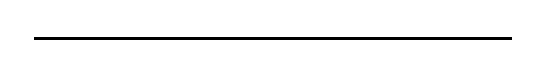
\begin{tikzpicture}
		\draw[thick, black] (0.25*\textwidth, 0) -- (0.75*\textwidth, 0);
		\node[rotate = 360 - 90, xshift = -0.6pt, yshift = 1pt] at (0.25*\textwidth,0){\decotwo};
		\node[rotate = 90, xshift = -0.6pt, yshift = 1pt] at (0.75*\textwidth,0){\decotwo};
	\end{tikzpicture}
	\end{center}
}

\pagestyle{fancy}

\newcommand{\lecday}[1][]
{
    \def\datee{#1}
    \fancyhead[L]{\datee}
}



\newcommand{\signature}
{
	\begin{tikzpicture}[remember picture,overlay]
		\node[fill = YellowOrange!20!white] at ([yshift = 1cm, xshift = -3cm]current page.south east) {\fontsize{10pt}{0pt}{\itshape Kara.$\mathcal{A}$}};
	\end{tikzpicture}
}

\AddToHook{shipout/background}{
  \begin{tikzpicture}[remember picture, overlay]
	  \node[] at ([yshift = 1.5cm,xshift = \textwidth /2 + 0.9cm]current page.south west) {\includegraphics[width = 0.5cm]{preview3}};
	  \node[] at ([yshift = 1.5cm,xshift = - \textwidth /2 - 0.9cm]current page.south east) {\includegraphics[width = 0.5cm]{preview4}};
  \end{tikzpicture}
}



\newtcolorbox[auto counter, number within = section]{remark}[1][]
{
       		title = Remark #1,
		enhanced,
		boxrule = 0pt,
		colback = white,
		breakable,
		arc = 4pt,
		colbacktitle = cyan,
		colback = cyan!5!white,
		segmentation style =
		{
			solid,cyan,thick,
		},
		attach boxed title to top left =
		{
			xshift = 0cm,
		},
		boxed title style =
		{
			boxrule = 0pt,
			sharp corners,
			drop fuzzy shadow = {cyan},
		},
		drop fuzzy shadow = {cyan!80!black},
}

\newtcolorbox[auto counter, number within = section]{theorem}[1][]
{                                      
		title = Theorem \thetcbcounter : #1,
		enhanced, 
		boxrule = 0pt,
		colback = white,
		breakable,
		arc = 4pt,
		colbacktitle = purple,
		colback = purple!5!white,
		segmentation style = 
		{
			solid, purple,thick,
		},
		attach boxed title to top left = 
		{
			xshift = 0cm, 
		},
		boxed title style = 
		{
			boxrule = 0pt,
			sharp corners,
			drop fuzzy shadow = {purple},
		},
		drop fuzzy shadow = {purple!80!black},
}

\newtcolorbox[auto counter, number within = section]{definition}[1][]
{                                      
		title = Definition \thetcbcounter : #1,
		enhanced, 
		boxrule = 0pt,
		colback = white,
		arc = 4pt,
		breakable,
		colbacktitle = YellowOrange!80!black,
		segmentation style = 
		{
			solid, YellowOrange,thick,
		},
		attach boxed title to top left = 
		{
			xshift = 0cm, 
		},
		colback = YellowOrange!5!white,
		boxed title style = 
		{
			boxrule = 0pt,
			sharp corners,
			drop fuzzy shadow = {YellowOrange!80!orange},
		},
		drop fuzzy shadow = {YellowOrange!80!black},
}

\newtcolorbox[auto counter, number within = section]{corollary}[1][]
{                                      
		title = corollary \thetcbcounter : #1,
		enhanced, 
		boxrule = 0pt,
		colback = white,
		arc = 4pt,
		breakable,
		colbacktitle = YellowOrange!80!black,
		segmentation style = 
		{
			solid, YellowOrange,thick,
		},
		attach boxed title to top left = 
		{
			xshift = 0cm, 
		},
		colback = YellowOrange!5!white,
		boxed title style = 
		{
			boxrule = 0pt,
			sharp corners,
			drop fuzzy shadow = {YellowOrange!80!orange},
		},
		drop fuzzy shadow = {YellowOrange!80!black},
}


\newtcolorbox{example}[1][]
{                                      
		title = Example,
		enhanced, 
		boxrule = 0pt,
		colback = white,
		arc = 4pt,
		segmentation style = 
		{
			solid, SpringGreen,thick,
		},
		breakable,
		colback = SpringGreen!5!white,
		colbacktitle = SpringGreen!80!black,
		attach boxed title to top left = 
		{
			xshift = 0cm, 
		},
		boxed title style = 
		{
			boxrule = 0pt,
			sharp corners,
			drop fuzzy shadow = {SpringGreen!80!orange},
		},
		drop fuzzy shadow = {SpringGreen!80!black},
}


\newcommand{\integral}[4]{\int\limits_{#1}^{#2} #4 d#3}
\newcommand{\limit}[3]{\lim\limits_{#1 \rightarrow #2} #3}
\newcommand{\strone}[2]{\left[ \begin{gathered}#1\\ #2\end{gathered} \right] }
\newcommand{\strtwo}[2]{\left\{ \begin{gathered}#1\\ #2\end{gathered} \right\} }
\newcommand{\strthree}[2]{\left\lfloor \begin{gathered}#1\\ #2\end{gathered} \right\rfloor }


\newcommand{\startbf}[1]{\text{\bfseries{#1}}}
\newcommand{\sett}[1]{\left\{ #1 \right\}}
\newcommand{\thesis}[1]{\left( #1 \right)}
\newcommand{\brkt}[1]{\left[ #1 \right]}
\newcommand{\floor}[1]{\left\lfloor #1 \right\rfloor}


\DeclareMathOperator{\img}{im} % Image
\DeclareMathOperator{\Img}{Im} % Image
\DeclareMathOperator{\coker}{coker} % Cokernel
\DeclareMathOperator{\Coker}{Coker} % Cokernel
\DeclareMathOperator{\Ker}{Ker} % Kernel
\DeclareMathOperator{\rank}{rank}
\DeclareMathOperator{\Spec}{Spec} % spectrum
\DeclareMathOperator{\Tr}{Tr} % trace
\DeclareMathOperator{\pr}{pr} % projection
\DeclareMathOperator{\ext}{ext} % extension
\DeclareMathOperator{\pred}{pred} % predecessor
\DeclareMathOperator{\dom}{dom} % domain
\DeclareMathOperator{\ran}{ran} % range
\DeclareMathOperator{\Hom}{Hom} % homomorphism
\DeclareMathOperator{\Mor}{Mor} % morphisms
\DeclareMathOperator{\End}{End} % endomorphism


\newcommand{\lm}{\ensuremath{\lambda}}
\newcommand{\eps}{\ensuremath{\epsilon}}
\newcommand{\veps}{\ensuremath{\varepsilon}}
\newcommand{\al}{\ensuremath{\alpha}}
\newcommand{\bb}{\ensuremath{\beta}}
\newcommand{\cc}{\ensuremath{\gamma}}
\newcommand{\dd}{\ensuremath{\delta}}
\newcommand{\DD}{\ensuremath{\Delta}}
\newcommand{\ff}{\ensuremath{\phi}}
\newcommand{\FF}{\ensuremath{\varphi}}

\newcommand{\RR}{\mathbb{R}}
\newcommand{\RO}{\mathcal{R}}
\newcommand{\EE}{\mathbb{E}}
\newcommand{\CC}{\mathbb{C}}
\newcommand{\RW}{\mathbb{R}^2}
\newcommand{\RT}{\mathbb{R}^3}
\newcommand{\RN}{\mathbb{R}^n}
\newcommand{\DS}{\mathcal{D}}

\newcommand{\KK}{\mathbb{K}}
\newcommand{\KW}{\mathbb{K}^2}
\newcommand{\KT}{\mathbb{K}^3}
\newcommand{\KN}{\mathbb{K}^n}

\newcommand{\NN}{\mathbb{N}}

\newcommand{\PS}{\mathcal{P}}
\newcommand{\AS}{\mathcal{E}}
\newcommand{\FS}{\mathcal{F}}
\newcommand{\LS}{\mathcal{L}}
\newcommand{\MS}{\mathcal{M}}


















\lecday[2025-02-11]

% \begin{document}

\section{Examples of norms of an infinite dimensional vector spaces}
let $a,b \in \RR $ with $a < b$. The $\RR $-vector space 
$E := \mathcal{C}^{0} \left( [a,b] , \RR  \right)$, 
(Constituted of continious real functions on 
$[a,b] $). can be equipped with several important norms, 
including  $\| . \|_{1}, \| . \| _{2}, \| . \| _{p} \quad 
\left( p \geq 1 \right)$, and $\| . \| _{\infty }$ defined by
\begin{align*}
	\| f \| _{1} &= 
	\int_{a}^{b} \left| f(t)  \right|dt  \\
	\| f \| _{2} &= 
	\sqrt{\int_{a}^{b} \left| f(t) ^2  \right|dt} 
	\\
	\| f \| _{p} &= 
	\left( 
		\int_{a}^{b} 
		\left| f(t)  \right|^{p}dt
	\right)^{1/p} \\
	\| f \| _{\infty } &=
	\sup_{t \in [a,b] } 
	\left| f(t)  \right| = 
	\max_{t \in [a,b] }\left| f(t)  \right|
\end{align*}
The norm $\| . \| _{2}$  is called the euclidean norm, the 
norm $\| . \| _{p}$ with $\left( p \geq 1 \right)$ is called
the Holder norm of exponent $p$ (or simply the $p$-norm), 
and the norm $\| . \| _{\infty }$ is called the uniform norm
say that a sequence of functions $(f_{n})_{n \in \NN}$, 
belonging to 
$\mathcal{C} ^{0} \left( [a,b] ,\RR  \right)$, converges to
$f \in \mathcal{C} ^{0}\left( [a,b] ,\RR  \right)$ in the 
sense of the norm 
$\| . \| _{\infty }$  is equivalent to say that 
$(f_{n})_{n \in \NN}$ converges uniformaly to 
$f$ on $[a,b]$, we can show that we have 
$\lim_{p \to \infty } \| . \| _{p} = \| . \|_{\infty }$ Further, 
it's important to note that these norms are not equivalent.
\begin{center}
	\textbf{Exercise : }
\end{center}
Show that $\| . \| _{p} \quad \left( p \geq 1 \right)$, is really
a norm on $E := \mathcal{C} ^{0} \left( [a,b], \RR \right)$. \\
\it Hint : Take inspiration from the solution of the previous exercise.
\normalfont
\section{Banach Spaces : }
\begin{definition}[]
A banach space is a normed $\KK$-vector space which is complete for the 
metric induced by it's norm.
\end{definition}
\begin{example}
In finite dimensional, let  $n \in \NN$ : 
\[
\RR -NVS \quad \left( \RR , \| . \|  \right) \quad 
\left( \RR ^n , \| . \| _{1} \right) \quad 
\left( 
	\RR ^n , \| . \| _{2}
\right) \quad 
\left( 
	\RR ^n , \| . \| _{\infty }
\right)
\]
they are all banach spaces, the same is for the :
\[
\CC -NVS \quad 
\left( \CC ,\| . \|  \right) \quad 
\left( 
	\CC ^n , \| . \| _{1}
\right)
\quad 
\left( 
	\CC ^{n}, \| . \| _{2}
\right) \quad 
\left( \CC ^n , \| . \| _{\infty } \right)
\]
Later, we will show a more general result stating that : 
\[
 \text{ \it Any finite-dimensional normal vector space is Banach } 
\]
\normalfont
\end{example}
\begin{theorem}[]
	The $\RR $-vector space 
	$E := \mathcal{C} ^{0} \left( [0,1] \right),\RR $, equipped
	with it's uniform norm $\| . \| _{\infty }$, is Banach.
\end{theorem}
\begin{proof}
We have to show that 
$\left( E, \| . \| _{\infty } \right)$ is complete, that is every
cauchy sequence of $\left( E, \| . \| _{\infty } \right)$ converges
in $\left( E, \| . \| _{\infty } \right)$, so let $(f_{n})_{n \in \NN}$ be
a cauchy sequence of $\left( E, \| . \|_{\infty }  \right)$ 
and let us show that it converges in $\left( E, \| . \| _{\infty } 
\right)$, By hypothesis, we have : 
\[
\forall \veps  > 0, \exists N \in \NN, 
\forall p,q \in \NN : \quad 
p > q > N \implies 
\| f_{p} - f_{q} \|  _{\infty } < \veps 
\]
that is (according to the definition of $\| . \|_{\infty } $ ) :
\[
\forall \veps  > 0, \exists N \in \NN, \forall p,q \in \NN :
\quad 
p > q > N \implies \sup_{x \in [0,1]}  
\left| f_{p} (x) - f_{q}(x)  \right| < \veps 
\]
or equivalently 
\[
\forall \veps  > 0, \exists N \in \NN,
\forall p , q \in \NN: \quad 
p > q > N \implies 
\forall x \in [0,1] : \quad 
\left| f_{p}(x) - f_{q}(x)  \right| < \veps 
\]
\end{proof}
Property $(1)$ shows that for all $x \in [0,1]$, the real sequence
$(f_{n})_{n \in \NN}$, is Cauchy in 
$\left( \RR , \| .\|  \right)$. But since is banach (i.e, complete) 
we derive that, for all $x \in [0,1]$, the real sequence 
$(f_{n})_{n \in \NN}$ converges in $\RR $, so we can define 
\[
\begin{array}{cccc}
	f : &  [0,1]  & \longrightarrow & \RR  \\

           &  x  & \longmapsto     & f(x) := \lim_{n \to \infty} f_{n} (x)   \\ 
\end{array}
\quad \left( \forall x \in [0,1] \right)
\]
on the other words, the sequence of functions $(f_{n})_{n \in \NN}$ 
converges pointwise to $f$. Now we are going to show that $f \in E$ and 
that $(f_{n})_{n \in \NN}$ converges in $\left( E, \| . \| _{\infty } \right)$ 
to $f$ (i.e., $(f_{n})_{n \in \NN}$ converges uniformally to $f$), by taking in 
$(1) $. 
\[
q = n > N \quad  \text{ and } \quad p \rightarrow  \infty 
\]
we will obtain : 
\[
\forall \veps  > 0,  \exists N \in \NN,  \forall n \in \NN : 
\quad n > N \implies 
\forall  x \in [0,1] : \quad \left| f_{n}(x) - f(x)  \right| < \veps 
\]
which is equivalent to 
\[
\forall \veps > 0, \exists N \in \NN, \forall n \in \NN : 
\quad n > N \implies 
\sup_{x \in [0,1]}  \left| f_{n}(x) - f(x)  \right| \leq \veps 
\]
Showing that, the sequence of functions $(f_{n})_{n \in \NN}$ converges uniformally
to $f$  on $[0,1]$. 
\divider 
\it Recall a theorem in \textbf{Analysis 3}, Let 
$(f_{n})_{n \in \NN}$ be a sequence of continiuous functions on a closed
interval $[a,b]$ where $(a,b \in \RR, a < b) $, that converges
uniformaly to a function $f$ on $[a,b]$. Then $f$ is also continuous 
on $[a,b]$.
\divider
\normalfont
By applying this result of analysis $3$, we derive that $f$ is also continuous
on $[0,1]$, that is $f \in E$, and $(f_{n})_{n \in \NN}$ is convergent
in $\left( E, \| . \| _{\infty } \right)$ to $f$, we conclude that 
$\left( \mathcal{C} ^{0} \left( [0,1] ,\RR \right), \| . \| _{\infty } \right)$ 
is Banach.  
\section{Bounded subset and bounded map on N.V.S : } 
The concepts of "bounded subsets" and "bounded maps" (or "bounded functions"), 
are in general defined in a metric space, however, the use of norms allows to
simplify them as stated by the following propositions : 
\begin{theorem}[]
A non empty subset $A$ of a N.V.S $E$ is bounded if and only if 
there is a positive real number $M$ such that : 
\[
\forall x \in A : \quad \| x \| \leq M
\]
\end{theorem}
\begin{proof}
	Let $E$ be a N.V.S and $A$ be a non empty subset of $E$. 
	\begin{center}
		(\textbf{ $ \implies $ })
	\end{center}
	Suppose that $A$ is bounded, that is $\dd \left( A \right) < +\infty $, 
	and let $x_0 \in  A$ be fixed. For all $x \in A$, we have 
	\begin{align*}
		\| x \| = \| x-x_0 + x_0 \|  & \leq 
		\| x-x_0 \| + \| x_0 \|  \\
					     & \leq 
					     \dd \left( A \right) + 
					     \| x_0 \| 
	\end{align*}
	So it sufficies to take $M = \dd \left( A \right) + \| x_0 \| $, to obtain
	the required property.
	\begin{center}
		(\textbf{ $ \impliedby $ })
	\end{center}
	Conversly, suppose that there exist $M > 0$ so that we have 
	\[
	\forall  x \in A : \quad \| x \| \leq M
	\]
	but this is equivalent to say that 
	\[
	A \subset \overline{B} \left( 0_{E}, M \right)
	\]
	implying that $A$ is bounded this completes the proof of the proposition
\end{proof}
\begin{theorem}[]
Let $X$ be a non empty set, $E$ be a N.V.S and 
\[
 f : X \longrightarrow E 
\]
be a map, then $f$ is bounded if and only if $\exists M > 0$ such that :
\[
\forall x \in X : \quad 
\| f(x)  \|  \leq M
\]
\end{theorem}
\begin{proof}
By definition, we say that $f$ is bounded, it's equivalent to say that 
$f \left( X \right)$ is bounded, which is equivalent to say (according
to the previous propsition), that $\exists M > 0$ such that : 
\[
\forall  y \in  f(X) : \quad 
\| y \|  \leq M
\]
equivalent to 
\[
\forall x \in  X : \quad 
\| f(x)  \|  \leq M
\]
This complets the proof.
\end{proof}
\chapter{Continious linear mappings between two N.V.S}
\begin{theorem}[Fundamental]
	Let $E$ and $F$ be two N.V.S on the same field $\KK = \RR \text{ or } \CC $,
	and $ f : E \longrightarrow F $, be a linear mapping then the following 
	properties are equivalent 
	\begin{enumerate}[(i)]
	\item  $f$ is continiuous on $E$ 
	\item $f$ is continious at the same $x_0 \in E$  
	\item $f$ is bounded on $\overline{B} \left( 0_{E},1 \right)$, i.e. : 
		\[
		\exists M > 0, \forall x \in  \overline{B}\left( 0_{E},1 \right) :
		\quad \| f(x)  \| _{F} \leq M
		\]
	\item   $f$ is bounded on $S \left( 0_{E},1 \right)$ 
	\item $\exists M > 0$ such that : 
		\[
			\forall x \in E : 
			\quad \| f(x)  \| _{F} \leq 
			M \| x \| _{E}
		\]
	\item $f$ is Lipchitz continious  
	\end{enumerate}
\end{theorem}
\begin{proof}
	We will show the following implications : 
	\[
		(i)  \implies 
		(ii)  \implies 
		(iii)  \implies 
		(iv)  \implies 
		(v)  \implies 
		(vi)  \implies 
		(i) 
	\]
	\divider 
	\begin{center}
		$(i) \implies (ii)  $ 
	\end{center}
	This is obvious 
	\divider 
	\begin{center}
		$(ii) \implies (iii)  $ 
	\end{center}
	Suppose that $f$ is continious 
	at some $x_0 \in E$, so $\exists \mu > 0$ such that : 
	\begin{equation}
		\forall x \in E : 
		\quad \| x-x_0 \|  < \mu \implies 
		\| f(x)  - f(x_0)  \|  _{F} < 1
	\end{equation}
	now, giving $y \in  \overline{B} \left( 0_{E},1 \right)$ arbitrary, 
	putting $x = \frac{\mu}{2}y + x_0$, we have : 
	\[
	\| x-x_0 \| _{E} = 
	\| \frac{\mu}{2}y \| _{E} = 
	\frac{\mu}{2} \| y \| _{E} \leq  \frac{\mu}{2} < \mu
	\]
	then $\| x-x_0 \| < \mu$, thus according to $(1)$ 
	$\| f(x) - f(x_0)  \| <  1$ but $f$ is linear 
	\begin{align*}
	\| f(x) - f(x_0)  \|_{F} = 
	\| f(x-x_0)  \| _{F} = 
	\| f \left( \frac{\mu}{2} y \right) \| _{F} &=
	 \| \frac{\mu}{2} f \left( y \right) \| _{F} \\
						    &= \frac{\mu}{2}
						    \| f \left( y \right) \| _{F}
	\end{align*}
	hence 
	\[
	\frac{\mu}{2} \| f(y)  \| _{F} < 1
	\]
	implying that 
	\[
	\| f(y)  \| _{F} < \frac{2}{\mu} \quad 
	\left( \forall  y \in \overline{B}\left( 0_{E},1 \right) \right)
	\]
	this shows that $f$ is bounded on $\overline{B}(0_{E},1) $ 
	\divider 
	\begin{center}
		$(iii) \implies (iv)  $ 
	\end{center}
	This is obvious since $S_{E} \left( 0_{E},1 \right) \subset 
	\overline{B}_{E} \left( 0_{E},1 \right)$, that is : 
	\[
	\exists M > 0, \forall u \in S_{E} \left( 0_{E},1 \right) : 
	\quad \| f(x)  \| _{F} \leq M
	\]
	so, for any $x \in  E \backslash \left\{ 0_{E} \right\}$, since
	$\frac{x}{\| x \|_{E} } \in S_{E} \left( 0_{E},1 \right)$, we have :
	\[
		\| f \left( \frac{x}{\| x \| _{E}} \right) \|  \leq 
		M 
	\]
	which gives 
	\[
	\| f(x)  \| _{F} \leq M \| x \| _{E}
	\]
	as required, remark that this last inequality is also valid for 
	$x= 0_{E}$ 
	\divider 
	\begin{center}
		$(iv) \implies (v)  $ 
	\end{center}
	Suppose that $\exists  M > 0$, satisfying the property : 
	\[
	\forall  x \in  E: \quad 
	\| f(x)  \| _{F} \leq M \| x \| _{E}
	\]
	then, for all $x,y  \in  E$, we have : 
	\[
	\| f(x) - f(y)  \| _{F} = \| f(x-y)  \|  \leq M \| \| x-y \|_{E} \| 
	\]
	implying that $f$ is $M$-Lipschitz
	\divider
	\begin{center}
		$(iv) \implies (v)  $ 
	\end{center}
	this is known to be true in metric spaces, (in general). This proof
	is complete
 \end{proof}
% \end{document}
